%% Term Paper for EEET2493_labreport_template.tex
%% V1.0
%% 2020/04/17
%% This is the template for a Term Paper following an IEEE paper. Modified by Krishna Tulsyan after Francisco Tovar after Michael Sheel original document.

%%*************************************************************************
%% Legal Notice:
%% This code is offered as-is without any warranty either expressed or
%% implied; without even the implied warranty of MERCHANTABILITY or
%% FITNESS FOR A PARTICULAR PURPOSE! 
%% User assumes all risk.
%% In no event shall the IEEE or any contributor to this code be liable for
%% any damages or losses, including, but not limited to, incidental,
%% consequential, or any other damages, resulting from the use or misuse
%% of any information contained here.
%%
%% All comments are the opinions of their respective authors and are not
%% necessarily endorsed by the IEEE.
%%
%% This work is distributed under the LaTeX Project Public License (LPPL)
%% ( http://www.latex-project.org/ ) version 1.3, and may be freely used,
%% distributed and modified. A copy of the LPPL, version 1.3, is included
%% in the base LaTeX documentation of all distributions of LaTeX released
%% 2003/12/01 or later.
%% Retain all contribution notices and credits.
%% ** Modified files should be clearly indicated as such, including  **
%% ** renaming them and changing author support contact information. **
%%*************************************************************************

\documentclass[journal]{IEEEtran}

% *** CITATION PACKAGES ***
\usepackage[style=ieee]{biblatex} 
\bibliography{example.bib}   
\usepackage{caption}
\usepackage{subcaption}


% *** MATH PACKAGES ***
\usepackage{amsmath}

% *** BLINDTEXT PACKAGE ***
\usepackage{blindtext}

% *** PDF, URL AND HYPERLINK PACKAGES ***
\usepackage{url}
% correct bad hyphenation here
\usepackage{graphicx}  %needed to include png, eps figures
\usepackage{float}  % used to fix location of images i.e.\begin{figure}[H]

\begin{document}

% paper title
\title{Second order methods in Training Neural Networks}

% author names 
\author{Avani Gupta, 2019121004}% <-this % stops a space
        

% make the title area
\maketitle

% As a general rule, do not put math, special symbols or citations
% in the abstract or keywords.
\begin{abstract}
In neural networks, second-order optimization is a step further from first-order optimization. In the training process of a neural network, additional curvature knowledge of an objective function is used to adaptively approximate the step-length of the optimization trajectory. It reduces training iteration and achieves rapid convergence even with less hyper-parameter tuning with the additional details.
Researchers are revisiting the advantages of second-order optimization approaches as memory allocation and processing resources increase. This paper provides an overview of second-order optimization methods for neural network training. It goes into the fundamentals of the Newton's methods, quasi-Newton, Gauss-Newton, and Levenberg-Marquardt, Approximate Greatest Descent and Hessian-Free optimization.  We perform several experiments and compare  first order method(Gradient Descent) with two second order methods(Levenberg Marquardt, Gauss Newton) on various parameters and analyse the viability and performance of optimization approaches.
\end{abstract}


\section{Introduction }
Neural Networks are used as function approximators which try to learn and predict the distribution of data. They are heavily used for various purposes like classification, machine translation, etc. \\
They have neurons with activation functions which work in unison. 
A neuron basically is a mathematical function which takes  inputs $x_{1}, x_{2}, x_{k}$. Each input has a corresponding weight value $w_{1}, w_{2}, w_{k}$. The output of neuron is given as $$f(x_{1}, x_{2}, x_{k}) = w_{1}*x_{1} + w_{2}*x_{2}+ w_{k}*x_{k}$$   where $x_{i}$ are the inputs to neuron.
During training, the loss is calculated and weights are updated via back-propagation. During testing the weights are fixed.
There are two types of optimization methods namely first and second order methods. The methods which use gradient information to construct the next training iteration are known as First-order methods. The methods which use Hessian to compute the iteration based on the optimization trajectory are known as Second-order methods \cite{battiti1992first}.

\begin{figure}%[tbhp]
\centering
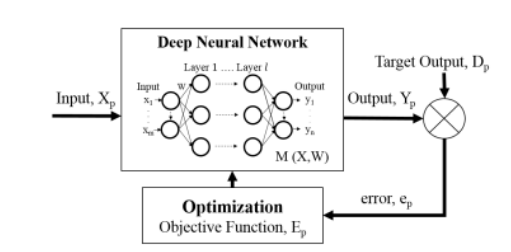
\includegraphics[width=.9\linewidth]{Figures/dl}
\caption{A typical Artificial Neural Network}
\label{table:Comparison}
\end{figure}


\section{Optimization in Neural Networks}
Back-propagation is a step in optimization techniques that measures error from the targeted and calculated performance. Optimization's aim is to minimize the target function, $E_{p}$, against the solution, W* for the minimum error value. The equation for iterative updates is as follows:
$ W_{k+1}=W_{k}+\alpha_{k} p_{k} $
where $W_{k+1}$ is the updated weight matrix, k is the iteration, $\alpha_{k}$ is the step length, and $p_{k}$ is the step direction. The gradient descent approach is one of the most widely used optimization methods in artificial neural network training. It uses first-order derivatives. The negative gradient is used to move across the error surfaces of gradient descent.
$$ -\frac{\partial E}{\partial W}=-\nabla E $$
The update equation can be written as, 
$$ W_{k+1}=W_{k}-\eta \frac{\partial E}{\partial W} $$

The choice of learning rate has a significant impact on gradient descent performance \ref{lr}. If the learning rate is too high, large steps are taken in each iteration and dramatic shifts are caused, it is often impossible to find the minimal point, W*.  A small learning rate observes too small steps and hence takes more epochs to reach the minima.

% Hence, it is a common practice to
% sweep through a few trials of η for hyperparameters fine-tuning. It is also known that ordinary
% gradient descent does not perform well in error surface in pathological curvature with multiple
% plateaus and saddle points. The second-order method with local curvature information is able
% to provide better trajectory across mountainous error surface commonly seen in artificial neural
% networks.
 \begin{figure}%[tbhp]
\centering
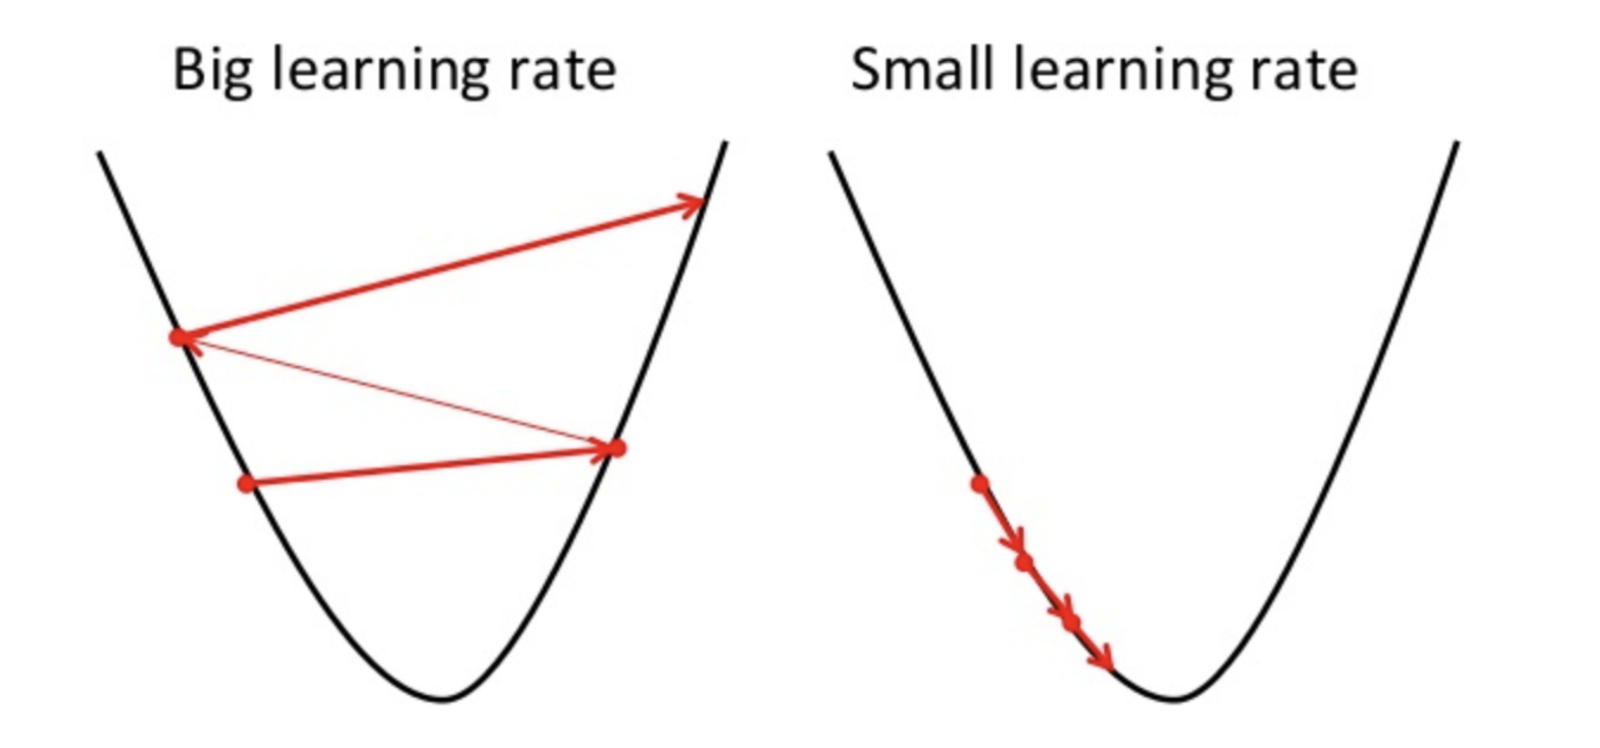
\includegraphics[width=.7\linewidth]{Figures/learning_rate}
\caption{Gradient Descent Steps depend on learning rate value:  if learning rate is large GD overshoots the minima; if small it takes small steps and a lot of time to converge;}
\label{lr}
\end{figure}

\section{Why should second-order optimization approaches help?}
First order methods require extensive fine-tuning of hyper-parameters since they rely on just the gradient information. The second order methods account the curvature of function and hence observe better performance. Essentially, second-order methods obtain the update direction by minimizing a quadratic approximate function. They follow the update rule given as: \\
$$ w_{k+1}=w_{k}-\alpha_{k} H_{k} \hat{\nabla} f\left(w_{k}\right) -(1)$$  \\
where $ H_{k}$ is Hessian's inverse or its approximation. \\
Since the large-scale neural networks require large number of parameters, the second-order methods approximate the calculation of equation (1). \\
\begin{figure}%[tbhp]
\centering
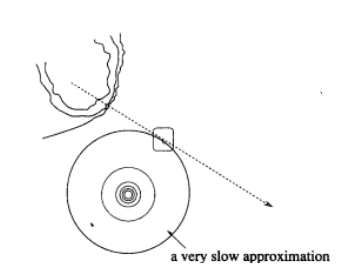
\includegraphics[width=.9\linewidth]{Figures/convergence}
\caption{First order methods don't take curvature information into account only rely on gradient information hence suffer from slow convergence}
\label{table:Comparison}
\end{figure}
Apart from this, non-linear optimization has issues like tightly coupled parameters with strong local dependencies, and large variations in scale along different directions in parameter space. First order methods like Gradient descent are very sensitive to above issues. For example it suffers from large oscillations and instability during training, which requires setting learning rate as inversely proportional to the size of the curvature along the highest curvature direction. These issues are addressed by second-order methods. Second-order optimization methods provide a much more powerful and elegant solution to the problem of variations in scale/curvature along different directions, by selectively re-scaling the gradient along different eigen-directions.

\section{Classification of Second Order methods }
Second-order methods can be classified into the following forms based on their approximations.

\subsection{Stochastic Inexact-Newton Methods}
Also known as "inexact-Newton method" this method computes exact Hessian inverse as ${H}_{k}$ but approximates $ \dot{H}_{k} \nabla f\left(w_{k}\right) $. A "Hessian-free" solution is suggested in \cite{martens2011learning}. Newton updates can be solved inexactly using Conjugate Gradient (CG), which computes the search path by adding CG to the Newton method and terminating it until it has made some progress, using hessian-vector products. \\ 
The majority of popular deep learning frameworks have an automated differentiation approach that can be used to rapidly compute Hessian-vector properties. \cite{wang2015confidence} proposed using a linear combination of current and past gradients instead of the regression to solve the Newton equation. In fact, this method does not outperform the simple inexact-Newton method.

\subsection{Stochastic Quasi-Newton Methods}
For large-scale machine learning, several stochastic quasi-Newton algorithms have recently been developed \cite{wang2017review}. These methods use an approximate hessian rather than a real one, and they derive curvature pairs using different parameters and update at different intervals. \\
The aim of Quasi-Newton methods is to achieve a lower per-iteration cost while still obtaining a reliable second-order estimation in order to achieve a better update per iteration. To prevent the updates phase from going unbounded, \cite{wang2017review} and \cite{curtis2017bfgs} revised the BFGS update rule. \\
When dealing with large-scale problems, \cite{gower2016stochastic} increases the reliability of the L-BFGS solution by decoupling parameter shifts from curvature estimation. \cite{keskar2016adaqn} took things a step further by adding additional testing requirements to ensure that the enhancement course is likely descendent. To approximate the information matrix, they often use an analytical fisher information matrix rather than a hessian matrix. \cite{ramamurthy2016sr1} proposed using rank one approximation in a restricted memory variant. Combining the L-SR1 solution with either the Line Search or Trust Region schemes optimises the model. It's worth noting that not all of the methods mentioned above are specifically formulated for non-convex problems.

\subsection{Stochastic Gauss-Newton methods}
A positive semi-definite approximation to the hessian matrix is the Gauss-Newton approximation. For multi-layer fully connected networks, an efficient block-diagonal approximation to the Gauss-Newton matrix is proposed in \cite{botev2017practical}. It is an estimate of the Kronecker Product that is factored to make estimation easier\cite{martens2015optimizing}. The difference is that it approximates the Fisher-information matrix rather than the hessian matrix. Since the network has layers that aren't fully linked and could have weight sharing, such as convolutional layers, using the Kronecker product structure to form the Gauss-Newton matrix is complicated. We did not equate this category because the emphasis of this article is on convolutional neural networks.


\subsection{Trust-Region Methods}
The trust area methods are another important class of second-order methods. Instead of solving the linear structure in (1), they get the update method by decreasing the quadratic approximation around the current solution with the norm constraints. To prevent the iterate from going too far, the trust area constraint, also known as the -norm constraint, is used. \\
However, trust area approaches for training deep networks have gained little attention because this non-convex quadratic sub-problem with bounded restriction is difficult to solve for large-scale applications. The cubic regularisation method \cite{nesterov2006cubic} solves a similar sub-problem to the trust area method, but instead of bounded limits, cubic regularisation replaces them.

\section{Second order Derivative methods for training of neural networks}
% \textbf{Table I: Iterative Optimization Methods}\\
% \begin{array}{lrl}\hline \text { Method } &  {\text { Step } \Delta \mathbf{x}} \\\hline \\ \text { Gradient Descent } & \Delta \mathbf{x}=-\alpha \mathbf{J_f}^{\top} \mathbf{f}(\mathbf{x}) \\\text { Newton's Method } & \left(\mathbf{H}^{\top} \mathbf{f}+\mathbf{J}^{\top} \mathbf{J}\right) \Delta \mathbf{x}= & -\mathbf{J}^{\top} \mathbf{f}(\mathbf{x}) \\\text { Gauss-Newton } & \mathbf{J}^{\top} \mathbf{J} \Delta \mathbf{x}= & -\mathbf{J}^{\top} \mathbf{f}(\mathbf{x}) \\\text { Levenberg-Marquardt } & \left(\mathbf{J}^{\top} \mathbf{J}+\lambda \mathbf{I}\right) \Delta \mathbf{x}= & -\mathbf{J}^{\top} \mathbf{f}(\mathbf{x})\end{array}


\subsection{Newton's Method}
It uses inverse Hessian matrices to compute the next update step.
$$ W_{k+1}=W_{k}-\eta\left(\nabla E_{k}+\beta_{k} p_{k-1}\right) $$
It usually takes just an iteration to reach the optima. It is thus very efficient. It has huge time O($N^3$) complexity per iteration and space complexity of order O($N^2$).
This is the reason being it bit much used for training large Neural Networks \cite{williams1989style}.  
This is overcome by Approximate Hessian methods.

\subsection{Conjugate gradient method}
It is an Approximate Hessian Method. This method does not compute actual Hessian. It computes the conjugate direction and adaptively alters the direction of descent in each iteration. The conjugate direction is computed as follows: 
$$ \beta_{k}=\frac{\left(\nabla E_{k}-\nabla E_{k-1}\right)^{T} \nabla E_{k}}{\left(\nabla E_{k-1}\right)^{T} \nabla E_{k-1}} $$ \\
The update rule thus is, \\
$$ W_{k+1}=W_{k}-\eta\left(\nabla E_{k}+\beta_{k} p_{k-1}\right) $$ 

Time complexity: O(N ) \\
It uses line search method to identify the step length and thus it is only suitable for batch learning.

\subsection{Quasi-Newton Method}
It computes updates using inverse Hessian estimation. The Broyden-Fletcher-Golfarb-Shanno (BFGS) algorithm is used for approximation \cite{loke1996rapid}. At each iteration, the approximation inverse Hessian, Q, for BFGS is determined using the following equation.  \\

$$ Q_{k}=\left(I-\frac{\delta \phi^{T}}{\phi^{T} \delta}\right) Q_{k-1}\left(I-\frac{\phi \delta^{T}}{\phi^{T} \delta}\right)+\frac{\delta \delta^{T}}{\phi^{T} \delta} $$ \\

where $ \delta=W_{k}-W_{k-1} $ and $ \phi=\nabla E_{k}-\nabla E_{k-1} $. \\
By substituting the estimated inverse Hessian into the update equation yields,
$$ W_{k+1}=W_{k}-\eta Q_{k} \frac{\partial E}{\partial w} $$ 
It has time complexity of order O($N^2$) but high space complexity O($N^2$) \\
Various algorithms have been proposed for reducing the space complexity. One of such algorithms is L-BFGS.

\subsection{L-BFGS}
By enforcing a "secant" (Quasi-Newton) condition, Quasi-Newton methods approximate the Hessian based on variations in gradients over many iterations. BFGS is one of common Quasi-Newton methods for estimating the Hessian in various ways. The BFGS Hessian approximation takes into account the entire history of gradients. If it takes only the most recent m gradients, it is called L-BFGS. \\
L-BFGS has the advantage of only storing the most recent m gradients, where m is normally between 5 and 20, which is a much smaller storage constraint than the n*(n+1)/2 elements needed by BFGS to store the maximum (triangle) of a Hessian estimate, where n is the problem dimension. \\
Unlike (full) BFGS, L-BFGS never specifically forms or stores the estimate of the Hessian (although some implementations of BFGS only form and update the Choelsky factor of the Hessian approximation, not the Hessian approximation itself); rather, the calculations that would be needed for the estimate of the Hessian are done without explicitly forming it. \\
For very large problems (when n is very large), L-BFGS is used instead of BFGS, although it does not do as well as BFGS. Where the memory needs of BFGS can be satisfied, BFGS is favoured over L-BFGS. L-BFGS might not be significantly worse than BFGS in terms of efficiency.

\subsection{Gauss Newton }
Gauss-Newton \cite{lecun2012efficient} method approximates inverse Hessian using the square of Jacobian(truncated Hessian) only,  ignoring the second-terms. Thus the equation for update can be written as: \\
$$ W_{k+1}=W_{k}-\eta\left(\frac{\partial E^{T}}{\partial W} \frac{\partial E}{\partial W}+\mu I\right)^{-1} \frac{\partial E}{\partial W} $$ \\

Time complexity is O($N^3$), all computation is done in each iteration and doesn't requires space/storage for next iteration.

\subsection{Levenberg Marquardt }
To tackle the problem of limitless Hessian, the Levenberg-Marquardt (LM) uses a regularisation parameter, with $\mu > 0$ . Levenberg-Marquardt method is written as follows: \\
$$ W_{k+1}=W_{k}-\eta\left(\frac{\partial E^{T}}{\partial W} \frac{\partial E}{\partial W}+\mu I\right)^{-1} \frac{\partial E}{\partial W} $$ \\
The parameter $\mu$ is also known as damping-factor.
When $\mu$ is small the updates tend towards Gauss-Newton and when  $\mu$ is large updates tend towards gradient descent. We set $u$ to a high value to ensure that the initial changes are small updates in the steepest-descent path \cite{gavin2019levenberg}.
However, adding a regularisation parameter is considered an ad-hoc solution, since it introduces another parameter that must be tuned for a successful learning trajectory.

% * Reduction in error → lambda divided by a factor of 10 & make the update.

% * Increase in error → lambda multiplied by a factor of 10 & reject update.

% When lambda is too small, it is essentially the same as Gauss Newton — will converge faster.


\subsection{LMAM Algorithm}
LMAM algorithm uses a "epoch-by-epoch" optimization approach to minimise cost function. At each epoch, the cost function must be decremented by $\delta Q_{t}$ to minimize E \cite{ampazis2002two}.
To first order, we can substitute the change in by its first differential and demand that 
$$ \boldsymbol{d} E\left(\boldsymbol{w}_{t}\right)=\delta Q_{\mathrm{t}}<0 $$ \\
Per epoch,$ \delta d_{w} $ is incremented by 
\\ $$ \boldsymbol{d} \boldsymbol{w}_{t}^{T} \nabla^{2} E\left(\boldsymbol{w}_{t}\right) \boldsymbol{d} \boldsymbol{w}_{t}=(\delta P)^{2} $$
\\ 
where $\delta_{P}$ is a small constant.
Thus the algorithm finds $ \delta Q_{t} $ in order to minimize the cost. In first order, we can substitute the change by its first differential and demand that $ d E\left(w_{t}\right)=\delta Q_{t}<0 $ \\
At each epoch of the learning process, the vector so that be incremented by  $ \delta W_{t} $ so that, 
$ \boldsymbol{d} \boldsymbol{w}_{t}^{T} \nabla^{2} E\left(\boldsymbol{w}_{t}\right) \boldsymbol{d} \boldsymbol{w}_{t}=(\delta P)^{2} $ \\
where $ \delta P $ is a small constant. As a result, the quest for a new optimum point in the space is limited to a narrow hyper-ellipse based on the current point. Gradient descent methods are considered to be inefficient due to the highly complicated shape of the cost function terrain, which typically consists of several flat areas and elongated small valleys. \\
Various techniques (including momentum) have been proposed to address the issue of reducing long hops when the gradient value is high while preventing movement deceleration when the gradient is very small.

\subsection{Approximate Greatest Descent method}
 AGD \cite{goh2011approximate} uses the trust area approach to find the smallest points depending on a set of boundaries. Unlike other approaches, AGD uses the true objective function rather than an approximate function to devise iteration steps. Let  $ Z_{1}, Z_{2},..., Z_{N}$ be the search boundaries. The search range is the lowest point on the original iteration, minus the last iteration. \\
The lowest point exists either in the interior or on the boundary of $Z_{N}$. The following is an LM-like approach derived from Taylor's series based on AGD: \\
$$ W_{k+1}=W_{k}-\eta(H+\mu I)^{-1} \frac{\partial E}{\partial W} $$ \\
where $ \mu=\|\nabla E\| / r $ is the relative step length. The radius, r, of the search boundaries is used to calculate the relative phase length. Unlike the LM process, AGD does not use any arbitrary parameters. 

\subsection{Hessian-free method}
\cite{martens2010deep} uses a scaled-down version of Hessian to calculate the local curvature before applying conjugate gradient to further optimise. \\
Since the complete Hessian is too large to compute at each iteration, the b with finite differences Hessian-free approach uses a scaled down version of the Hessian matrix, H, at the expense of one extra gradient evaluation via the identity. \\
$$ \hat{H}=\lim _{\epsilon \rightarrow 0} \frac{\nabla E(w+\epsilon)-\nabla E(w)}{\epsilon} $$ 
The Hessian approximation used for the Hessian-free approach optimises the quadratic goals equation using only matrix-vector products. However, it only functions by using a conjugate gradient. Along with the training iterations, the action of conjugate gradient would inevitably allow substantial improvement in minimization.

\section{Experimentation}
We compare Gradient Descent, Gauss Newton and Levenberg Marquardt algorithms by experimenting extensively (Code) \footnote{\url{https://colab.research.google.com/drive/1sHeR5j1R_gd8vVBN_Mm51R201fOVdWLx?usp=sharing}}. In our experiments we use the algorithm to fit a Gaussian. Starting from an initial estimate, we aim to use the optimization algorithms to reach the optima(required Gaussian) using least squares error formulation.
Thus our formulation is Simple Non-Linear least squares for Gaussian function. \\
The equation of Gaussian Distribution is given as follows: 
$$ p(x)= a* e^{-\frac{1}{2}\left(\frac{x-m}{s}\right)^{2}} $$
where $a = \frac{1}{\sigma \sqrt{2 \pi}}$, m is mean of gaussian and s is the standard deviation.
The numbers a, m, and s are variables to be estimated.
We start with their initial estimates and then apply the algorithms to find their optimum values for the gaussian.
The Gradient Descent, Gauss Newton and LM converge for above values of learning rate and tolerance in given estimate of $s_{gt} = 20$, $a_{est} = 10$, $m_{est} = 13$, $s_{est} = 19.12$ and 50 observations.

\textbf{Hyper-parameter settings} \\
We extensively perform hyper-parameter tuning for first order method (GD) and minor tuning for second order methods(GN/LM) and find the following setting of hyper-parameters to give the most optimal performance. 
\begin{itemize}
\item \textbf{Learning rate} 0.01 for Gradient Descent and Gauss Newton, 10 for LM (experimentally found: see graphs above)
\item \textbf{Tolerance} 1e-2 for Gradient Descent, Gauss Newton and LM 
\item \textbf{Damping factor for LM}: 1.1 (note: this is intentionally kept 1.1 since if decrease in loss learning rate should decrease so that we are more probable to not miss the local optima. And for increase in loss it is intended to increase learning rate since algorithm is going farther away from optima(or shooting it). 
Also, the authors of LM algorithm \cite{gavin2019levenberg} suggested to use damping factor greater than one. \\
\end{itemize}

\begin{figure}%[tbhp]
\centering
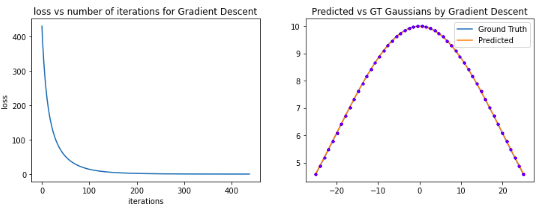
\includegraphics[width=.9\linewidth]{Figures/GD}
\caption{Gradient Descent performance}
\label{table:Comparison}

\centering
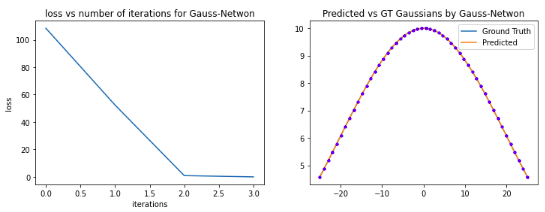
\includegraphics[width=.9\linewidth]{Figures/GN}
\caption{Gauss Newton performance}
\label{table:Comparison}


\centering
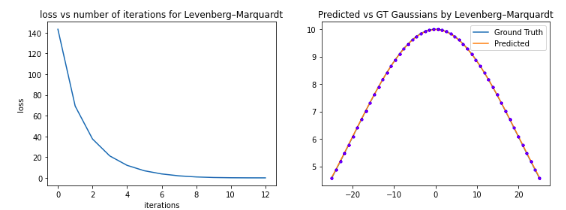
\includegraphics[width=.9\linewidth]{Figures/LM}
\caption{Levenberg Marquardt performance}
\label{table:Comparison}
\end{figure}
\textbf{Observations}
\begin{itemize}
\item \textbf{Gradient Descent is hugely dependent on learning rate parameter and needs intensive tuning}\\
If the learning rate is too high or too small, the Gradient descent algorithm doesn't converge.
With a small learning rate, the Gradient Descent algorithm takes long time to converge. If we use too large a learning rate, the gradient descent algorithm might overshoot the minima and keep on oscillating. 

\item \textbf{Different initial estimate}\\
We vary the initial estimates of a, m, and s from the ground truth to check how far off initialization can a particular algorithm handle (figure \ref{diff_init_esti}). We observe the following:
\begin{itemize}
    \item Gauss Newton and Levenberg Marquardt converge for initial estimates which are relatively far from the Ground Truth.
    \item Gradient Descent on the other hand is not able to converge for far off estimates but converges for medium to low changes to initial estimates. 
    \item The Levenberg-Marquardt method acts more like a gradient-descent method when the parameters are far from their optimal value, and acts more like the Gauss-Newton method when the parameters are close to their optimal value.
\end{itemize} 
% \begin{figure}%[tbhp]
% \centering
% \includegraphics[width=.9\linewidth]
% {Figures/diff_init_esti}
% \caption{Different Initial Estimate: performance of algorithms. $for a_est: 20.0  m_est: 13.0  s_est: 19.2$}
% \label{table:Comparison}
% \end{figure}

\begin{figure}%[tbhp]
\centering
\begin{subfigure}[b]{0.5\textwidth}
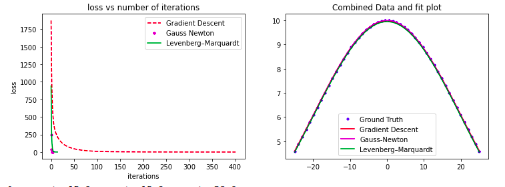
\includegraphics[width=.9\linewidth]
{Figures/diff_init_esti}
\caption{ for $a_{est}: 20.0$,  $m_{est}: 13.0$ and  $s_{est}: 19.2$}
\end{subfigure}

\begin{subfigure}[b]{0.5\textwidth}
\centering
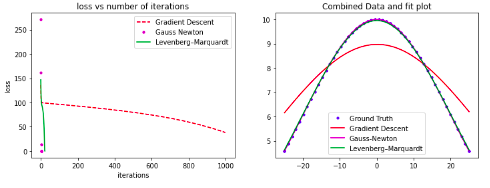
\includegraphics[width=.9\linewidth]
{Figures/gd_doesnt_converge}
\caption{ for $a_{est}: 10.0$,  $m_{est}: 5.0$ and  $s_{est}: 45.0$}
\end{subfigure}
 \hfill

\caption{Comparison of algorithms for different Initial estimate}
\label{diff_init_esti}
\end{figure}

\item \textbf{Different number of samples} \\
We vary the number of samples in gaussian distribution and try to predict the gaussian from the three algorithms (figure \ref{diff_obs}).\\ We observe that the Levenberg Marquardt and Gauss Newton algorithms can handle even small number of observations whereas Gradient Descent needs a large sample population.
\begin{figure}%[tbhp]
\centering
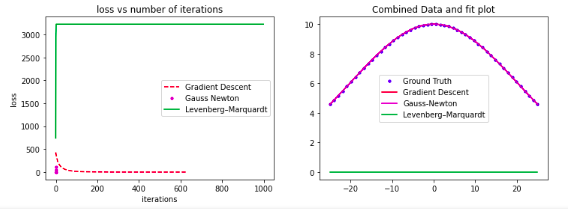
\includegraphics[width=.9\linewidth]
{Figures/comparison}
\caption{Comparison for tolerance 0.0001}
\label{table:Comparison}
\end{figure}

\begin{figure}%[tbhp]
    \centering
    \begin{subfigure}[b]{0.5\textwidth}
    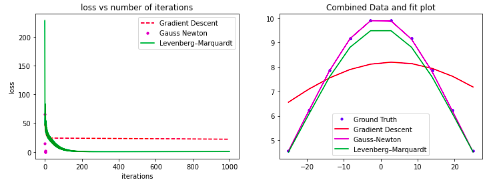
\includegraphics[width=.9\linewidth]
    {Figures/10_obs}
    \caption{10 samples}
    \label{table:Comparison}
    \end{subfigure}
    \hfill
    
    \begin{subfigure}[b]{0.5\textwidth}
    \centering
    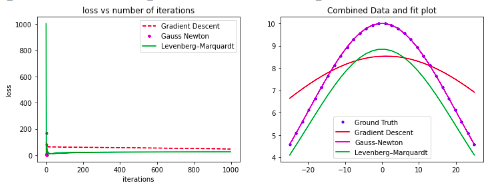
\includegraphics[width=1\linewidth]
    {Figures/30_obs}
    \caption{30 samples}
    \end{subfigure}
    \hfill
     
    \begin{subfigure}[b]{0.5\textwidth}
    \centering
    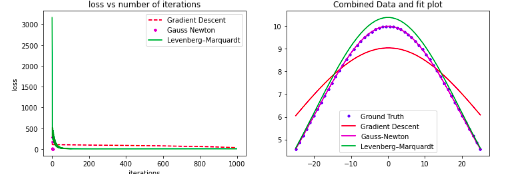
\includegraphics[width=.9\linewidth]
    {Figures/52_obs}
    \caption{52 samples}
    \end{subfigure}
    
    \caption{Comparison of algorithms for different number of observations available}
    \label{diff_obs}
\end{figure}


    \begin{itemize}
    \item The Gradient Descent, Gauss Newton and LM converge for above values of learning rate and tolerance in given estimate.
     \item Gradient descent is not able to converge on small number of observations since gradient steps are much smaller based on learning rate, whereas the steps in GN and LM are much larger.
    \end{itemize}

\item \textbf{Number of iterations to converge}
\begin{itemize}
    \item The Gauss-Newton(GN) and Levenberg-Marquardt(LM) typically converge much faster than gradient-descent(GD) methods. This is attributed to fact that former take larger steps than GD. 
    \item Larger steps are desired if loss is increased since the algorithms prediction is far from optima and smaller steps are desired when loss is decreased attributing to fact that algorithm is near optima(so that it doesn't overshoot the optima). 
    \item This is achieved by Levenberg-Marquardt algorithm by changing learning rate dynamically according to loss incurred. Thus LM takes larger steps when far away from optima and smaller steps when it is close to optima and hence converges better. 
\end{itemize}

    
\item \textbf{Noisy Objective function}
 \begin{itemize}
 \item For higher levels of noise LM performs best.
 \item For medium noise only LM and Gauss Newton converge.
 \item For low noise all converge, given learning rate and tolerance are fixed. This is due to fact that LM and GN takes larger steps and hence don't get stuck at optima which is incurred due to noise in GD.
 \end{itemize}

\item \textbf{Learning rate}
\begin{itemize}
\item When learning rate is  is decreased, the Levenberg-Marquardt method approaches the Gauss-Newton method, and the solution typically accelerates to the local minimum.
\item The gradient descent doesn't converge on larger learning rates since it overshoots the minima and may oscillate. 
\item When initial learning rate is too small(<1; for damping factor of 1.1) Levenberg-Marquardt doesn't converge for 1000 iterations whereas Gauss newton does converge.
\item However we found that on increasing learning rate along with increasing tolerance, Levenberg-Marquardt converges in less iterations than Gauss Newton. \\

\end{itemize}
\end{itemize}

Thus to conclude our order of superiority of algorithms (from most cases above) is 
$$ LM > GN > GD $$ 
This is intuitive too since Levenberg-Marquardt theoretically combines pros of Gauss Newton and Gradient Descent. 
 

\begin{figure}%[tbhp]
\centering
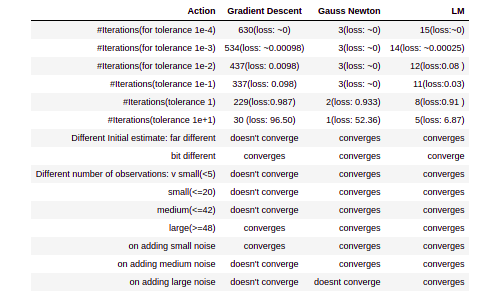
\includegraphics[width=1\linewidth]{Figures/table2}
\caption{Comparison of Gradient Descent, Gauss Newton and LM algorithm}
\label{table:Comparison}
\end{figure}

\section{Comparison Analysis}
 Gradient descent is prone to local minima. Gradient descent also needs extensive hyper-parameter fine-tuning. \\
 
 \begin{figure}%[tbhp]
\centering
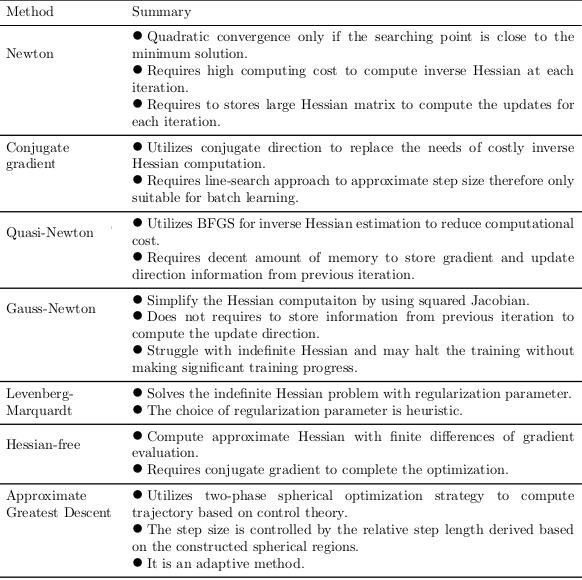
\includegraphics[width=1\linewidth]{Figures/summary}
\caption{Summary of Algorithms}
\label{Comparison}
\end{figure}


 The benefits and drawbacks of second-order derivatives approaches are outlined in Table.\ref{Comparison}. The Newton method employs quadratic structures, which have a high computational expense and necessitate the storage of a massive Hessian matrix for computation. Due to the seemingly vast number of parameters in deep neural network, the ordinary Newton approach is difficult to apply to artificial neural network training. Conjugate gradient uses a line-search technique to approximate phase lengths, but it's only useful for batch training. Quasi-Newton uses approximate Hessian to solve the computational problem. However, since the BFGS approach relies on gradient knowledge from previous iterations, it is also susceptible to memory problems. While Gauss-Newton algorithms do not require storing information from previous iterations, they are vulnerable to gradient explosion if the matrix is not positive definite. By adding the regularisation parameter to contain the infinite Hessian proclivity, the LM procedure introduced an ad-hoc approach.

Since the regularisation alternative is not well-theorized, the LM approach also necessitates certain hyper-parameter fine-tuning. The Hessian-free method suggested a clever approach to Hessian estimation, but it can only be used with conjugate gradient as the second stage of the algorithm.
For adaptive second-order methods, AGD is one of the most recent Algorithms. The multistage optimal control scheme has influenced and inspired it. As a result, a two-phase spherical optimization technique with relative step length is used. As the step length is modified according to the state of preparation, AGD is free of disappearing and bursting gradients. The relative phase length is a natural adaptive optimization method that performs similarly to first-order optimization methods. AGD uses gradient knowledge to build an adaptive phase length that can be used to cope with various stages of an optimization problem, making the search for optimal trajectories easier.

\section{Conclusion}
Second order methods take into account the curvature information and hence are able to converge better and faster compared to  First Order methods. Second order methods are categorised into Stochastic Inexact-Newton Methods, Stochastic Quasi-Newton Methods, Stochastic Gauss-Newton methods and Trust-Region Methods. We discussed Newton's Method, Conjugate Gradient Method, Gauss Newton Method, Levenberg Marquardt, Approximate Greatest Descent method and Hessian-free methods in above paper. 

The Newton's method was the first second-order optimization method proposed for neural networks training. It uses full Hessian in training and is prone to computation and memory issues. \\
Quasi-Newton and Gauss-Newton were introduced to counter the drawback of Newton method with truncated Hessian and approximate Hessian respectively. Levenberg-Marquardt method was proposed to solve the indefinite matrix problem by introducing a regularization parameter to the truncated Hessian's. Consequently, Approximate Greatest Descent utilizes control theory in developing a two-phase long term and short term optimization approach. The Hessian-free method was then proposed as an alternative second-order optimization technique with the help of Conjugate Gradient algorithm. \\
Conjugate Gradient and Quasi-Newton both require to store information from previous iteration. On the other hand, Hessian-free method on Hessian approximation does not work as efficient without Conjugate Gradient algorithm. Although Gauss-Newton and Levenberg-Marquardt method require more computation power per iterations, this can be addressed with parallel processing. Levenberg-Marquardt also uses less memory compared to other Hessian approximation approaches which enables the algorithm to run on lower-ends graphical processing unit. Approximate greatest descent utilizes adaptive two phase methods which have been proven to provide better trajectory towards the minimum.

\printbibliography
\end{document}


